%%%%%%%%%%%%%%%%%%%%%% section 4%%%%%%%%%%%%%%%%%%%%%
\section{Le syst\`eme $M/M/1$}
Nous allons maintenant discuter du système de file d'attente non trivial le plus simple.  
\subsection{Principes fondamentaux} Un syst\`eme de file d'attente $M/M/1/\textrm{GD}/\infty/\infty$  dispose d'intervalles d'arrivée et de temps de service dont les distributions respectives sont exponentielles, et un serveur unique. On peut le modéliser \`a l'aide d'un processus de naissance et de mort o\`u
\begin{align*}
\lambda_{j} &= \lambda, \ j=0,1,2,\ldots \\ 
\mu_{0} &= 0 \\
\mu_{j} &= \mu,\  j=1,2,3,\ldots 
\end{align*}
En substituant ces taux de natalit\'e et de mortalit\'e dans (\ref{eq:ssbr}), on obtient  
$$\pi_{j} = \frac{\lambda^{j} \pi_{0}}{\mu^{j}}=\rho^j \pi_0,$$ o\`u $\rho = \lambda/\mu$ repr\'esente l'\textbf{l'intensité du trafic} dans le syst\`eme. \newpage\noindent 
Étant donné que le système doit se trouver exactement dans l'un des \'etats à tout moment, la somme de toutes les probabilités se doit d'\^etre $1$: $$\pi_{0}+\pi_1 + \pi_2+\cdots = \pi_0(1+\rho+\rho^{2}+\cdots ) = 1.$$
Lorsque $0 \leq \rho < 1$, la s\'erie converge vers $\frac{1}{1-\rho}$, d'o\`u l'on d\'erive $$\pi_{0}\cdot \frac{1}{1-\rho} = 1 \implies \pi_0 = 1-\rho \implies \pi_{j} = \rho^{j} \pi_0 = \rho^j (1-\rho);$$
c'est la \textbf{probabilit\'e de retrouver le syst\`eme  dans le  $j^{\text{e}}$ \'etat dans le r\'egime stable}. Si au contraire $\rho \geq 1$, la s\'erie diverge et le syst\`eme n'atteint pas de r\'egime stable. Intuitivement, cela se produit lorsque $\lambda \geq \mu$: lorsque le taux d'arrivée est supérieur au taux de service, l'état du système croît sans cesse et la file d'attente ne se d\'egage jamais.
\newl À partir de maintenant, nous allons présumer que $\rho < 1$ afin de garantir l'existence des probabilités  $\pi_{j}$ dans le r\'egime stable, à partir desquelles nous pouvons déterminer plusieurs quantités d'intérêt. \par En supposant que l'état d'équilibre a été atteint, on peut montrer que $L$, $L_{s}$, et $L_{q}$ sont, respectivement:
\begin{align*}
L &= \frac{\lambda}{\mu - \lambda}=\frac{\rho}{1-\rho}\\
L_{s} &= \rho\\
 L_{q} &= \frac{\rho^{2}}{1-\rho}.
 \end{align*}
\`A l'aide de la loi de Little, nous pouvons également obtenir $W$, $W_{s}$, et $W_{q}$ en divisant chacune des valeurs correspondantes de $L$ par~$\lambda$:
\begin{align*}
W &= \frac{1}{\mu - \lambda}\\
W_{s} &= \frac{1}{\mu}\\
W_{q} &= \frac{\lambda}{\mu(\mu-\lambda)}.
 \end{align*}
On note comme prévu que $W,W_q\to +\infty$ quand $\rho\to 1$. En revanche, $W_{q}\to 0$ et $W\to \frac{1}{\mu}$ (le \textbf{temps moyen de service}) comme $\rho\to 0$.
\begin{Exemple} (selon \cite{QS_W}) En moyenne, dix clients arrivent à un guichet \`a toutes les heures. Si le client moyen est servi en 4 minutes, et si les intervalles d'arriv\'ee et le temps de service suivent tous deux des distributions exponentielles, alors: \begin{itemize}[noitemsep]
	\item[(a)] Quelle est la probabilité que le guichet se retrouve au repos? 
	\item[(b)] Sans compter le client qui se fait servir, combien de clients font la queue au guichet, en moyenne? \item[(c)] Combien de temps, en moyenne, un client passe-t-il dans le syst\`eme de file d'attente (y compris le temps de service)?
	\item[(d)] En moyenne, combien de clients seront servis par le caissier \`a chaque heure?
\end{itemize}
\textbf{Solution:} nous faisons affaire \`a un syst\`eme de file d'attente $$M/M/1/\textrm{GD}/\infty/\infty$$ pour lequel $\lambda = 10$ clients/h et $\mu = 15$ clients/h, d'o\`u   $\rho = 10/15 = 2/3$.
\begin{itemize}[noitemsep]
	\item[(a)] Puisque  $\pi_{0} = 1 - \rho = 1/3$, le guichet se retrouve au repos $1/3$ du temps.  
	\item[(b)] Il y a $L_{q} = \rho^{2}/(1-\rho) = 4/3$ clients en ligne pour le guichet, en moyenne. 
	\item[(c)] On sait que $L = \lambda/(\mu - \lambda) = 10/(15-10) = 2$,, d'o\`u  $W = L/\lambda = 0.2 \textrm{ h} = 12 \textrm{ min}$.
	\item[(d)] Si le guichet est toujours occupé, on sert en moyenne $\mu=15$ clients par heure. Selon (a), nous savons que la caissière n'est occupée que les deux tiers du temps, c'est-\`a-dire qu'\`a chaque heure, elle ne sert en moyenne que $15  \cdot 2/3 = 10 $ clients. C'est un résultat raisonnable car, dans le régime stable, $10$ clients entrent dans le syst\`eme  et $10$ clients quittent le syst\`eme \`a chaque heure.
\end{itemize}
\end{Exemple}
\begin{Exemple} (selon \cite{QS_E}) Supposons que tous les propriétaires de voitures fassent le plein lorsque leur réservoir est exactement à moitié vide. Supposons \'egalement que $7.5$ clients arrivent en moyenne \`a chaque heure à une station-service qui n'a qu'une seule pompe et qu'il faut en moyenne $4$ minutes par voiture pour faire le plein. Supposons finalement que les intervalles d'arriv\'ees et les temps de service suivent tous deux des distributions exponentielles. \begin{itemize}[noitemsep]
	\item[(a)] Quelles valeurs prennent $L$ et $W$ dans ce sc\'enario? 
	\item[(b)] Supposons que lorsqu'il y a pénurie de gaz, les achats d'essence se fassent dans la panique. On modélise ce phénomène en imaginant que tous les propriétaires de voitures achètent désormais de l'essence lorsque leur réservoir est rempli aux trois quarts exactement. Comme chaque propriétaire de voiture met désormais moins d'essence dans le réservoir à chaque visite à la station, nous supposons que la durée moyenne du temps de service  a été réduite à $10/3$ minutes. De quelle fa\c{c}on est-ce que cela affecte les valeurs de $L$ et $W$?
\end{itemize}
\textbf{Solution:} on prend pour acquis que le syst\`me de file d'attente prend la forme $$M/M/1/\textrm{GD}/\infty/\infty,$$ o\`u $\lambda = 7.5$ voitures/h et $\mu = 60/4 = 15$ voitures/h.  Nous avons alors $\rho = 7.5/15 = 1/2$.
\begin{enumerate}[noitemsep]
	\item[(a)] Par définition, $L = \lambda/(\mu - \lambda) = 7.5/(15-7.5) = 1$ et $W = 1/7.5 \approx 0,13$ h $=7.8$ min. Dans cette situation, tout est sous contrôle et de longues files d'attente semblent peu probables.
\item[(b)] Pour le sc\'enario o\`u les achats se font dans la panique,   $\lambda = 2(7.5)=15$ voiture/h puisque les propri\'etaires de voiture font le plein 2 fois plus souvent qu'au pr\'ealable, et $\mu = 60 \cdot 3 /10  = 18$ voitures/h, d'o\`u $\rho = \lambda/\mu = 5/6$. Dans ce cas,   
$$ L = \frac{\rho}{1-\rho} = 5 \text{ voitures, et } W = \frac{L}{\lambda} = \frac{5}{15} = 20 \text{ min}.$$
Ainsi, les achats dans la panique ont pour effet de plus que doubler le temps d'attente dans la file d'attente.
\end{enumerate}
\end{Exemple}
\noindent In a $M/M/1$ queueing system, we have $$L=\frac{\rho}{1-\rho}=-1+\frac{1}{1-\rho}, $$ and it is easy to see that $L\to\infty$ as $\rho\to 1$. The $5-$fold increase in $L$ when $\rho$ jumps from $1/2$ to $5/6$ (with accompanying jumps in $W$) illustrate that fact. 
\subsection{Limited Capacity}
In the real world, queues never become infinite -- they are limited due to requirements of {space} and/or {time}, or service operating policy. Such a queuing model falls under the purview of \textbf{finite queues}. \par Finite queue models restrict the number of customers allowed in the service system. Let $N$ represent the maximum allowable number of customers in the system. If the system is at \textbf{capacity}, the arrival of a $(N+1)^{\textrm{th}}$ customer results in a failure to enter the queue -- the customer is assumed balk and depart without seeking service.\newl Finite queues can also be modeled as a birth-death process, but with a slight modification in its parameters:  with these parameters:
\begin{align*}
\lambda_{j} &= \lambda, \ j=0,1,2,\ldots,N-1 \\ 
\lambda_{N} &= 0,\ \mu_{0} = 0 \\
\mu_{j} &= \mu,\  j=1,2,3,\ldots, N 
\end{align*}
The restriction $\lambda_{N} = 0$ is what sets this model apart from the $M/M/1/\infty$. It makes it impossible to reach a state greater than $N$. Because of this restriction, a steady-state always exist because even if $\lambda \geq \mu$, there can never be more than $N$ customers in the system.
\newl Mathematically, this has the effect of replacing the infinite series linking the $\pi_j$'s by a finite geometric series, which always converges: 
$$ \pi_{0}+\pi_1 + +\cdots + \pi_N = \pi_0(1+\rho+\cdots +\rho^{N}) = 1,$$ from which we can derive \begin{align*}\pi_{0}\cdot \frac{1-\rho^{N+1}}{1-\rho} = 1 &\implies \pi_0 = \frac{1-\rho}{1-\rho^{N+1}} \\ &\implies \pi_{j} = \begin{cases}\rho^{j} \frac{1-\rho}{1-\rho^{N+1}} & \text{for $j=0,\ldots,N$} \\ 0 & \text{for $j>N$}\end{cases}\end{align*}
Since $L = \sum^{N}_{j=0} j\cdot \pi_{j}$ (why?), 
$$L = \frac{\rho [1+ N \rho^{N+1} - (N+1) \rho^{N} ]}{(1-\rho)\left(1-\rho^{N+1}\right)} $$
when $\lambda\neq\mu$. \newl As in the $M/M/1/\infty$ queue, $L_{s} = 1 - \pi_{0}$, and $L_{q} = L - L_{s}$.  \newpage\noindent In a finite capacity model, only $\lambda - \lambda \pi_{N} = \lambda\left(1-\pi_{N}\right)$ arrivals per unit time  actually enter the system on average ($\lambda$ arrive, but $\lambda\pi_N$ find the system full). With this fact, 
$$ W = \frac{L}{\lambda\left(1-\pi_{N}\right)}\quad \text{and}\quad W_{q} = \frac{L_{q}}{\lambda\left(1-\pi_{N}\right)}.$$
What does that look like in practice? 
\begin{Exemple} Consider a one-man barber shop with a total of 10 seats. Assume, as has always been the case so far (but need not be), that inter-arrival times are exponentially distributed with an average of 20 prospective customers arriving each hour at the shop. Those customers who find the shop full do not enter (perhaps they do not like standing). The barber takes an average of 12 minutes to cut each customer's hair; assume that haircut times are also exponentially distributed.
\begin{itemize}[noitemsep]
	\item[(a)] On average, how many haircuts per hour will the barber complete?
	\item[(b)] On average, how much time will be spent in the shop by a customer who enters?
\end{itemize}
\textbf{Solution:} there is not that much to say. Let's dive in!
\begin{itemize}[noitemsep]
	\item[(a)] A fraction $\pi_{10}$ of all arrivals will find the shop full. Thus, an average of $\lambda\left(1-\pi_{10}\right)$ will actually enter the shop each hour.  All entering customers receive a haircut, so the barber will give an average of $\lambda\left(1-\pi_{10}\right)$ haircuts per hour. In this scenario, $N=10$, $\lambda=20$ customers/hr, and $\mu=60/12 = 5 $ customers/hr. Thus $\rho= 20/5 = 4$ and  we have 
	\begin{align*} \pi_{0} &= \frac{1-\rho}{1-\rho^{N+1}} = \frac{1-4}{1-4^{11}}\approx 7.15\times 10^{-7}  \text{ and} \\ \pi_{10} &= 4^{10} \pi_{0} = \frac{3}{4} \text{ (from formula in opposite column)}.\end{align*}
Thus, an average of $20(1 - 3/4)= 5$ customers per hour will receive haircuts. This means that an average of $20 - 5 = 15$ prospective customers per hour will not enter the shop.	
\item[(b)] To determine $W$, we must first compute 
$$L = \frac{4 [1+ (10) 4^{11} - (11) 4^{10} ]}{(1-4)\left(1-4^{11}\right)} = 9.67.$$ 
Using the formulas described above, we obtain 
$$ W = \frac{L}{\lambda\left(1-\pi_{10}\right)} = \frac{9.67}{5} = 1.93 \text{ hr}.$$
This barber shop is crowded -- the barber would be well-advised to hire at least one more barber!
\end{itemize}
\end{Exemple}
\noindent What \textit{would} be the effect of hiring a second barber? In order to answer this question, we will study $M/M/c$ queueing systems.   
%%%%%%%%%%%_________Section 5____________%%%%%%%%%%%%%%%%%%%%
\begin{figure*}[!t]
\centering
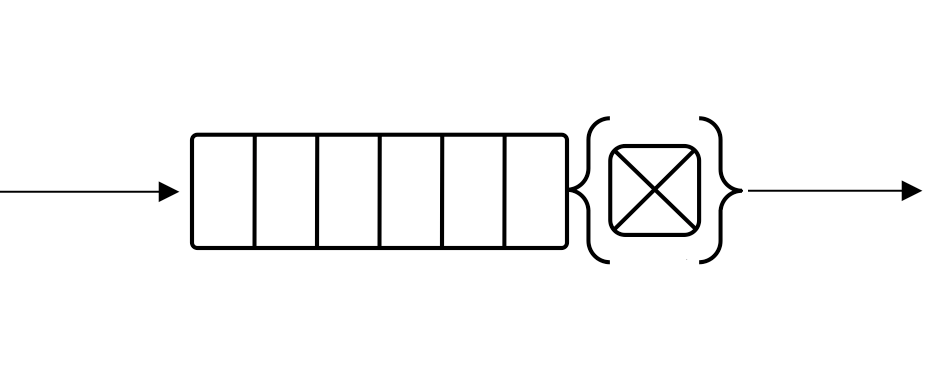
\includegraphics[width=0.45\textwidth]{Images/MM12.png}\qquad\qquad 
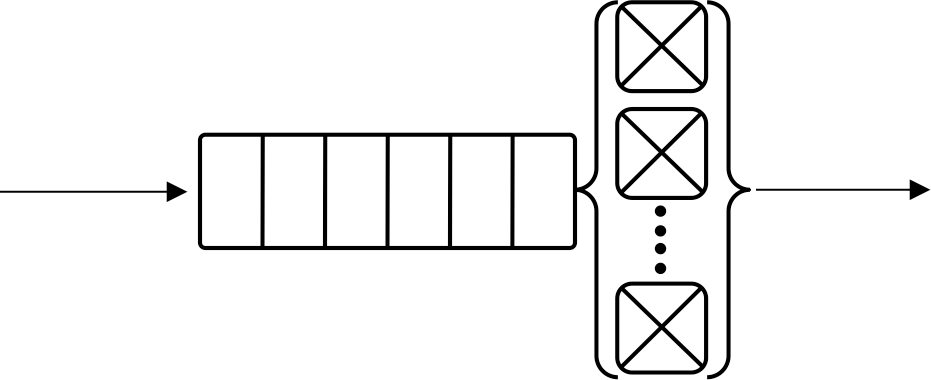
\includegraphics[width=0.45\textwidth]{Images/MMc.png}\\
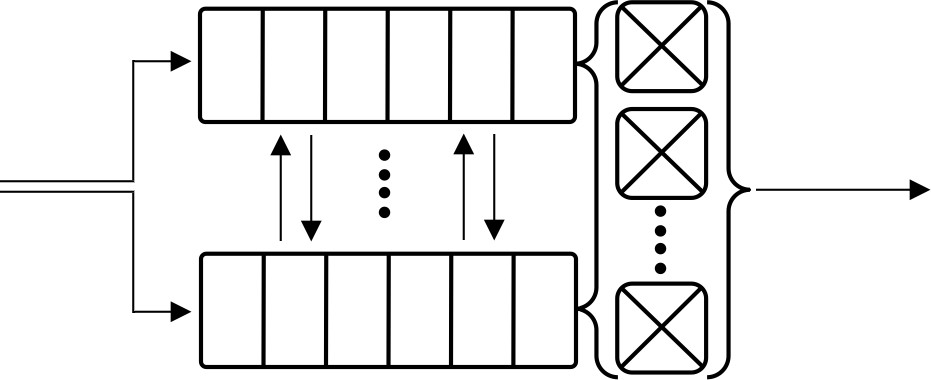
\includegraphics[width=0.45\textwidth]{Images/Tandem.png}
\caption{\small Schematics of various queueing systems ($M/M/1$, $M/M/c$, tandem); customers arrive from the left, enter the queue and progress through it until they are served, at which point the exit the queue.}\label{fig:MM}\hrule
\end{figure*}\afterpage{\FloatBarrier}
